\documentclass[12pt,a4paper]{article}

\usepackage[a4paper,margin=1in]{geometry}
\usepackage{graphicx}
\usepackage{booktabs}
\usepackage{amsmath,amssymb}
\usepackage{float}
\usepackage{hyperref}
\usepackage{xcolor}
\usepackage{listings}
\usepackage{enumitem}
\usepackage{fancyhdr}
\usepackage{longtable}
\usepackage{subcaption}   % required for the 2-graphs-per-row layout
\usepackage{mathptmx}     % Times New Roman substitute font (text + math)
\usepackage{fontawesome} % for using icons

\hypersetup{colorlinks=true,linkcolor=blue,urlcolor=blue}

\pagestyle{fancy}
\fancyhf{}
\lhead{ICS1512}
\rhead{Machine Learning Algorithms Laboratory}
\cfoot{\thepage}

\lstset{
language=Python,
basicstyle=\ttfamily\small,
numbers=left,
frame=single,
breaklines=true,
showstringspaces=false
}

\begin{document}

\begin{tabular}{|p{4cm}|p{11cm}|}
\hline
Experiment No. & 2\\ \hline
Experiment Title & Email Spam/Ham Classification using Na\"{\i}ve Bayes and KNN
\href{https://github.com/Poojashree81/ICS1512-Machine-Learning-Laboratory.git}{\faGithub} \\ \hline
Student Name & Poojashree V \\ \hline
Register Number & 3122247001043 \\ \hline
Faculty & Dr. Poreddy Ajay Kumar Reddy \\ \hline
Submission Date & 14th July 2026\\ \hline
\end{tabular}

\section{Objective}
This experiment builds spam classifiers for the Spambase e-mail dataset using Na\"ive Bayes and K-Nearest Neighbours (KNN), and compares how the two families perform against each other. We evaluate the Gaussian, Multinomial, and Bernoulli variants of Na\"ive Bayes on the same train/test split so their relative strengths can be judged fairly. For KNN, we look at how varying the number of neighbours ($k$) changes classification accuracy, and try to pin down a reasonable value of $k$ for this data. We also compare KDTree and BallTree, the two data structures commonly used to speed up neighbour search in KNN, and check whether \texttt{GridSearchCV} or \texttt{RandomizedSearchCV} does a better job tuning KNN's hyperparameters. Finally, we look at both the theoretical and the actually-measured training/prediction times for each algorithm, and validate everything with 5-fold cross-validation rather than trusting a single split.


\section{Problem Statement}
Each e-mail in this dataset is represented as a 57-dimensional numeric feature vector: 48 relative frequencies of specific words (\texttt{word\_freq\_*}), 6 relative frequencies of specific characters (\texttt{char\_freq\_*}), and 3 statistics describing runs of consecutive capital letters (\texttt{capital\_run\_length\_*}). The task is to predict the binary label \texttt{class} $\in \{0,1\}$, where $1$ means \emph{spam} and $0$ means \emph{ham} (a legitimate e-mail). This is a standard supervised, binary classification problem, and we build two quite different families of classifiers to attack it: a generative probabilistic model (Na\"{\i}ve Bayes, in three flavours suited to different assumptions about the features) and a non-parametric, instance-based model (KNN). The point of this report isn't really to chase the single highest accuracy number -- it's to understand \emph{why} each algorithm behaves the way it does on this particular feature space, and how choices like distance metric, neighbour-search structure, and hyperparameter search strategy trade accuracy off against computational cost.

\section{Dataset Description}

\begingroup
\small
\begin{longtable}{|p{6cm}|p{8cm}|}
\hline
Dataset Name & Spambase Dataset \\ \hline

Dataset Source & Kaggle -- \url{https://www.kaggle.com/datasets/somesh24/spambase} (mirror of the UCI Machine Learning Repository Spambase dataset) \\ \hline

Number of Samples & 4601 e-mail instances \\ \hline

Number of Features & 57 numeric features (48 \texttt{word\_freq\_*}, 6 \texttt{char\_freq\_*}, 3 \texttt{capital\_run\_length\_*}) \\ \hline

Number of Classes & 2 -- \texttt{class}~$=1$ (spam), \texttt{class}~$=0$ (ham). This matches the classic Spambase composition of 1{,}813 spam ($\approx$39.4\%) and 2{,}788 ham ($\approx$60.6\%) instances, which lines up with the 4601-row count we loaded and is visible in the class-distribution plot in Section~4. \\ \hline

Missing Values & None found -- \texttt{df.info()} reported 4601 non-null entries across all 58 columns. Even so, the pipeline still coerces every feature column to numeric with \texttt{pd.to\_numeric(..., errors="coerce")} and fills any resulting \texttt{NaN} with the column median, mainly as a safeguard. In practice this step turned out to be a no-op on the real data. \\ \hline

Train-Test Split & 80\% / 20\% stratified split (\texttt{train\_test\_split}, \texttt{random\_state=42}, \texttt{stratify=y}) $\rightarrow$ 3680 training samples, 921 test samples, keeping the 39.4\%/60.6\% class ratio consistent in both. \\ \hline

\end{longtable}
\endgroup


\section{Exploratory Data Analysis}

\subsection{Class Distribution}
\begin{figure}[H]
\centering
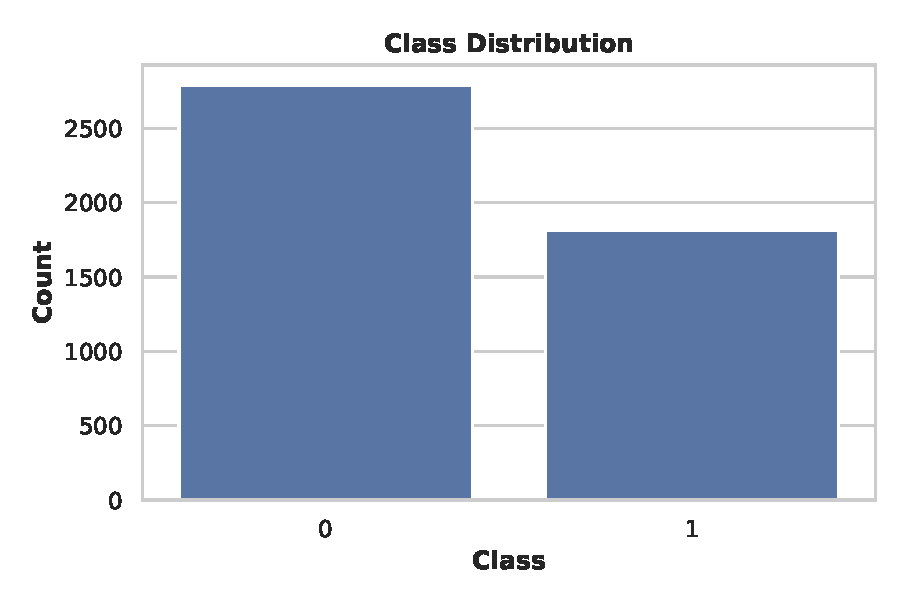
\includegraphics[width=0.6\linewidth]{figures/class_distribution.eps}
\caption{Class distribution of the Spambase dataset (0 = ham, 1 = spam).}
\end{figure}
\textbf{Inference:} From Figure 1 we can see the dataset is moderately imbalanced, with ham outnumbering spam by roughly 3:2. That's not severe enough to make raw accuracy meaningless, but it's also not something to ignore -- a classifier that just predicted ``ham'' every time would already land close to 60\% accuracy without learning anything. That's exactly why we track Precision, Recall, F1 and ROC-AUC alongside accuracy for every model in this report. It ends up mattering most for Bernoulli NB (Section~8.1), whose raw accuracy of 0.6482 is barely above that trivial baseline once you look closely.

\subsection{Correlation Heatmap}
\begin{figure}[H]
\centering
\includegraphics[width=0.85\linewidth]{figures/correlation_heatmap.eps}
\caption{Pearson correlation heatmap across all 58 columns of the preprocessed dataset.}
\end{figure}
\textbf{Inference:} Looking at Figure 2, the 48 \texttt{word\_freq\_*} columns and the 6 \texttt{char\_freq\_*} columns each seem to form a loosely correlated block. That's not too surprising -- promotional/spam vocabulary (words like ``free'', ``money'', ``credit'') tends to show up together in the same messages. The three \texttt{capital\_run\_length\_*} features are much more tightly correlated with each other, which makes sense since all three are really just different ways of describing bursts of capitalisation, so they carry a fair bit of overlapping rather than independent information. We also notice that no single feature correlates strongly with the \texttt{class} label on its own -- correlations are weak-to-moderate across the board. That's actually favourable for Na\"{\i}ve Bayes' conditional-independence assumption, but it also explains why no individual feature is a reliable spam signal by itself; the model has to combine a lot of weak signals to get anywhere.
 
\subsection{Feature Distributions (Top-4 Correlated Features)}
The four features most strongly correlated (by absolute value) with the target label turned out to be \texttt{word\_freq\_your}, \texttt{word\_freq\_000}, \texttt{word\_freq\_remove} and \texttt{char\_freq\_\%24} (the frequency of the `\$' character; it's stored as \texttt{\%24}, its percent-encoded form, in the source CSV column header).

\begin{figure}[H]
\centering
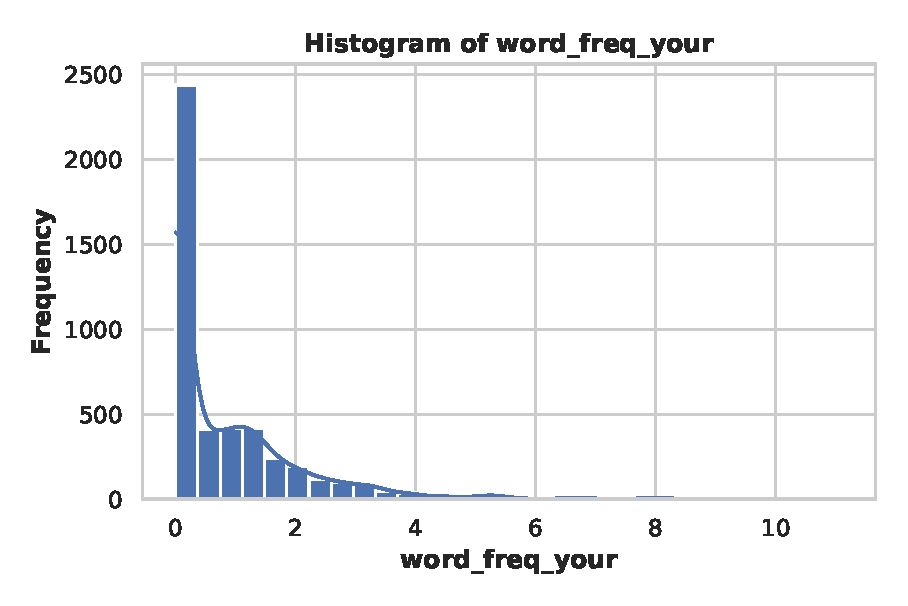
\includegraphics[width=0.48\linewidth]{figures/histogram_word_freq_your.eps}
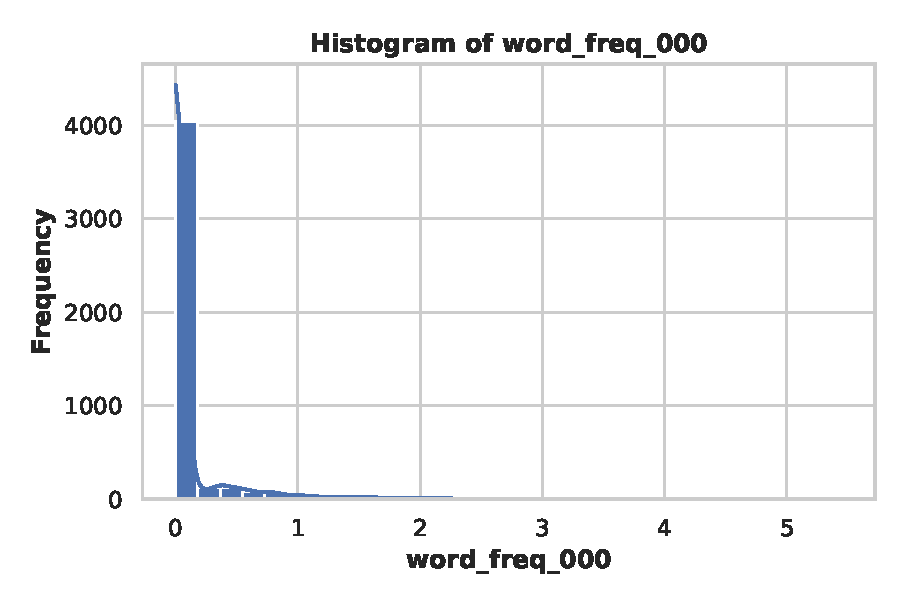
\includegraphics[width=0.48\linewidth]{figures/histogram_word_freq_000.eps}
\caption{Histograms of \texttt{word\_freq\_your} and \texttt{word\_freq\_000}.}
\end{figure}
\begin{figure}[H]
\centering
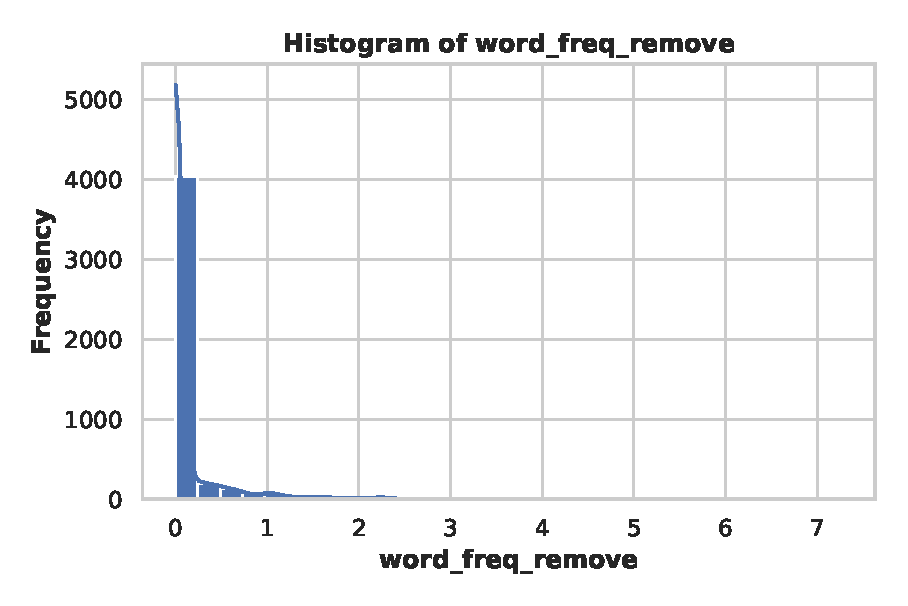
\includegraphics[width=0.48\linewidth]{figures/histogram_word_freq_remove.eps}
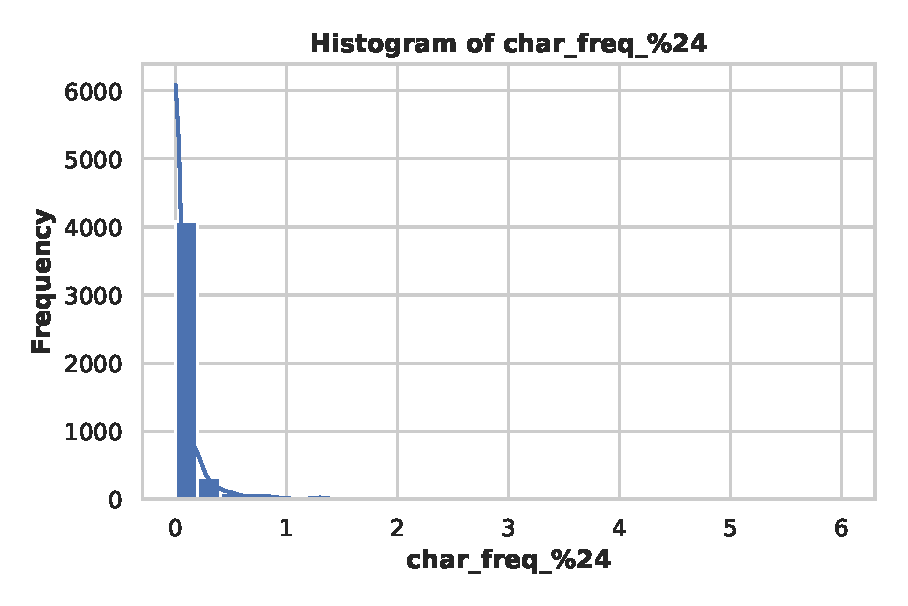
\includegraphics[width=0.48\linewidth]{figures/histogram_char_freq__24.eps}
\caption{Histograms of \texttt{word\_freq\_remove} and \texttt{char\_freq\_\%24}.}
\end{figure}
\textbf{Inference:} All four distributions here are heavily right-skewed and zero-inflated -- most e-mails contain each of these tokens/characters 0\% of the time, with only a small tail of messages using them repeatedly. This is a rough match for what GaussianNB assumes (a per-class normal distribution), and it's probably why Gaussian NB over-predicts spam -- high recall (0.9532) but weak precision (0.7178), which we see later in Section~8.1. It's arguably worse for BernoulliNB. Since almost every value sits far below the fixed 0.5 binarisation threshold, even in messages that are genuinely spammy, the binarised features collapse to 0 for most instances. One likely explanation for Bernoulli NB's very low recall (0.1295) is exactly this -- the threshold wipes out the signal that made these features useful in the first place.

\begin{figure}[H]
\centering
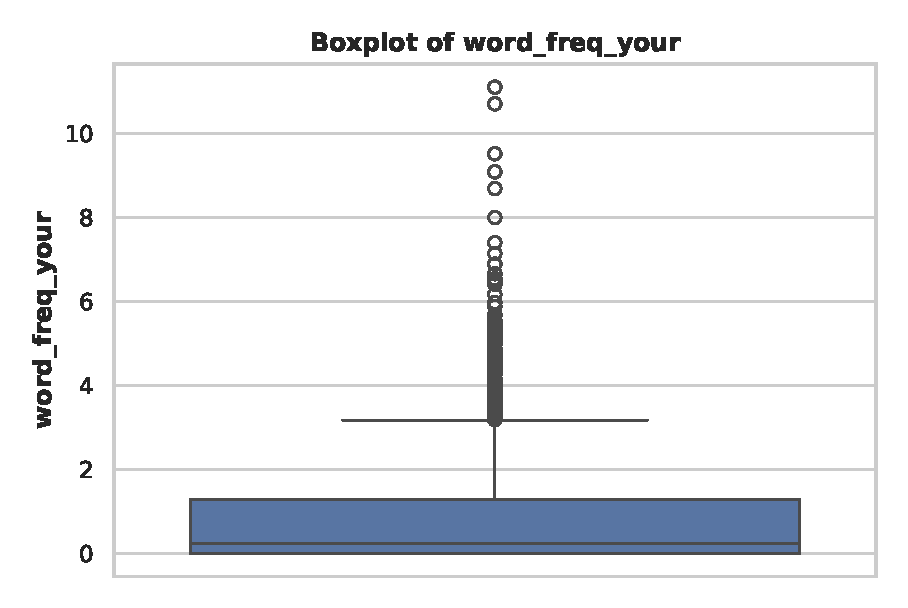
\includegraphics[width=0.48\linewidth]{figures/boxplot_word_freq_your.eps}
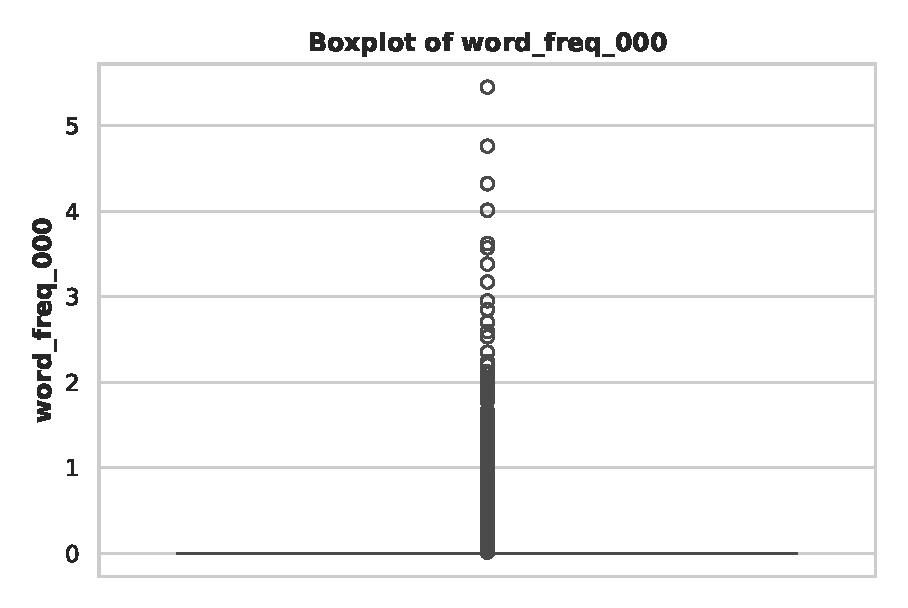
\includegraphics[width=0.48\linewidth]{figures/boxplot_word_freq_000.eps}
\caption{Boxplots of \texttt{word\_freq\_your} and \texttt{word\_freq\_000}.}
\end{figure}
\begin{figure}[H]
\centering
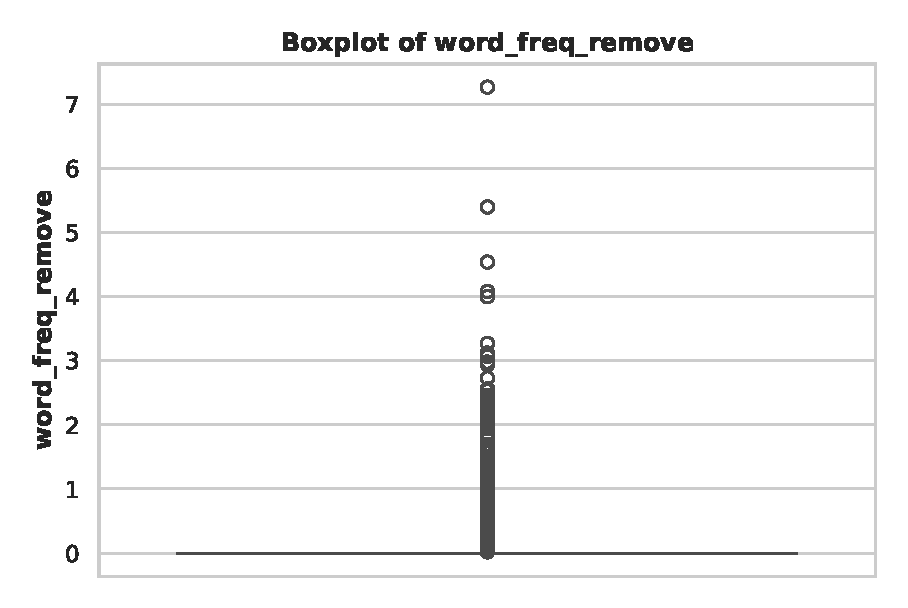
\includegraphics[width=0.48\linewidth]{figures/boxplot_word_freq_remove.eps}
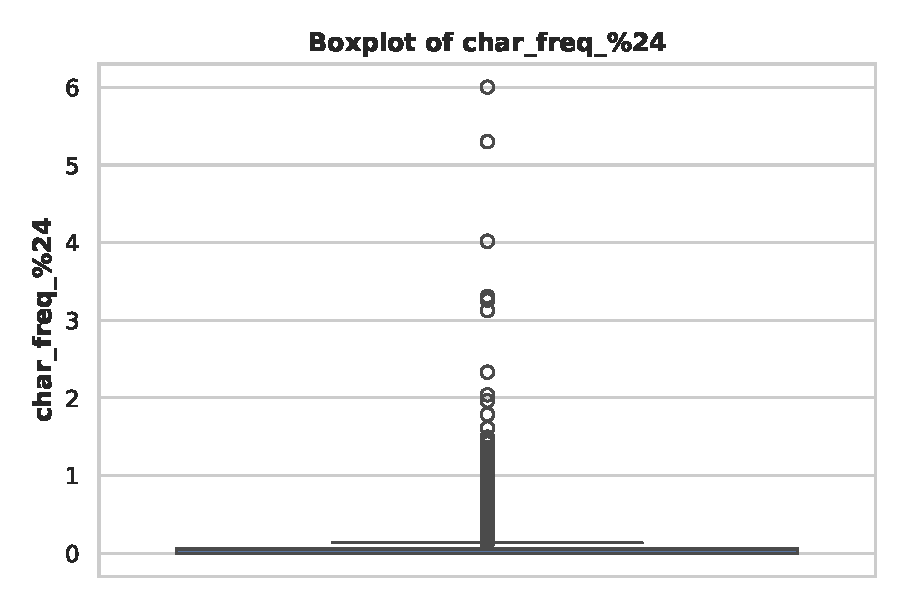
\includegraphics[width=0.48\linewidth]{figures/boxplot_char_freq__24.eps}
\caption{Boxplots of \texttt{word\_freq\_remove} and \texttt{char\_freq\_\%24}.}
\end{figure}
\textbf{Inference:} These boxplots back up what we saw in the histograms -- the interquartile box for each of these four features sits squeezed near zero, with a long tail of outliers stretching well past the upper whisker. We were tempted to treat those outliers as noise, but they're not; they're basically the spam messages that repeatedly use ``your'', numeric strings, the word ``remove'' (common in fake unsubscribe text), and the `\$' symbol (common in monetary spam). So we left them in and didn't trim anything before modelling.


\section{Data Preprocessing}
\begin{itemize}
\item \textbf{Missing value handling:} We coerced feature columns to numeric (\texttt{errors="coerce"}) and filled any resulting \texttt{NaN} with the column median. The target column would have been label-encoded if it were non-numeric, but that wasn't needed here since \texttt{class} was already integer-typed. As noted in Section~3, the raw data had no missing values anyway, so this step was really just a safety net.
\item \textbf{Encoding:} Not needed -- all 57 features and the target are already numeric.
\item \textbf{Feature scaling:} We applied \texttt{MinMaxScaler} (scaling every feature to $[0,1]$) inside the pipeline for every model except Gaussian NB, which works directly on the raw feature scale since it just estimates a per-class mean and variance rather than depending on distance or non-negative counts. Scaling matters a lot for Multinomial NB (which needs non-negative inputs), for Bernoulli NB (whose \texttt{Binarizer(threshold=0.5)} step needs a bounded $[0,1]$ range), and for all KNN variants, where distance would otherwise be dominated by the large-magnitude \texttt{capital\_run\_length\_*} features.
\item \textbf{Train-test split:} 80/20 stratified split, \texttt{random\_state=42}, as described in Section~3.
\item \textbf{Feature engineering:} None beyond scaling/binarising -- we used the raw 57 Spambase features as they came.
\end{itemize}


\section{Code Implementation}
The core building blocks of the pipeline are shown below (the full code is in the accompanying notebook).
 
\subsection*{Preprocessing}
\begin{lstlisting}
target_col = df.columns[-1]
if df[target_col].dtype == "object":
    le = LabelEncoder()
    df[target_col] = le.fit_transform(df[target_col])
 
for col in df.columns[:-1]:
    df[col] = pd.to_numeric(df[col], errors="coerce")
df = df.fillna(df.median(numeric_only=True))
\end{lstlisting}
 
\subsection*{Unified Evaluation Function}
\begin{lstlisting}
def evaluate_pipeline(model, name, X_train, X_test, y_train, y_test, make_plots=True):
    start_train = time.perf_counter()
    model.fit(X_train, y_train)
    train_time = time.perf_counter() - start_train
 
    start_pred = time.perf_counter()
    y_pred = model.predict(X_test)
    pred_time = time.perf_counter() - start_pred
 
    y_score = model.predict_proba(X_test)[:, 1] if hasattr(model, "predict_proba") \
              else model.decision_function(X_test)
 
    acc  = accuracy_score(y_test, y_pred)
    prec = precision_score(y_test, y_pred, zero_division=0)
    rec  = recall_score(y_test, y_pred, zero_division=0)
    f1   = f1_score(y_test, y_pred, zero_division=0)
    auc  = roc_auc_score(y_test, y_score)
    return {"Model": name, "Accuracy": acc, "Precision": prec, "Recall": rec,
            "F1-Score": f1, "ROC-AUC": auc, "Train Time (s)": train_time,
            "Pred Time (s)": pred_time}
\end{lstlisting}
 
\subsection*{Model Pipelines}
\begin{lstlisting}
gaussian_model = Pipeline([("clf", GaussianNB())])
multinomial_model = Pipeline([("scaler", MinMaxScaler()), ("clf", MultinomialNB())])
bernoulli_model = Pipeline([
    ("scaler", MinMaxScaler()),
    ("bin", Binarizer(threshold=0.5)),
    ("clf", BernoulliNB())
])
\end{lstlisting}
 
\subsection*{Hyperparameter Search Space (KNN)}
\begin{lstlisting}
param_grid = {
    "clf__n_neighbors": [1, 3, 5, 7, 9, 11],
    "clf__weights": ["uniform", "distance"],
    "clf__algorithm": ["brute", "kd_tree", "ball_tree"],
    "clf__metric": ["minkowski"],
    "clf__p": [1, 2]
}
\end{lstlisting}


\section{Machine Learning Algorithm}
\subsection{Na\"{\i}ve Bayes}
Na\"{\i}ve Bayes is a generative probabilistic classifier built on Bayes' theorem, with the simplifying (``na\"{\i}ve'') assumption that features are conditionally independent given the class:
\[
P(C \mid X) = \frac{P(X \mid C)\,P(C)}{P(X)}, \qquad P(X \mid C) = \prod_{i=1}^{d} P(x_i \mid C)
\]
The predicted class is $\hat{C} = \arg\max_{C} P(C)\prod_{i=1}^{d}P(x_i\mid C)$. The three variants we use here only differ in what form $P(x_i \mid C)$ is assumed to take:
\begin{itemize}[leftmargin=*]
\item \textbf{Gaussian NB:} assumes $x_i \mid C \sim \mathcal{N}(\mu_C,\sigma_C^2)$, i.e.\ $P(x_i\mid C)=\frac{1}{\sqrt{2\pi\sigma_C^2}}\exp\!\left(-\frac{(x_i-\mu_C)^2}{2\sigma_C^2}\right)$. Works best for continuous, roughly bell-shaped features.
\item \textbf{Multinomial NB:} treats features as if they're counts/frequencies drawn from a multinomial distribution, $P(x\mid C)\propto\prod_i p_{C,i}^{x_i}$ (with Laplace smoothing). This tends to suit word-frequency-style features such as \texttt{word\_freq\_*} quite well.
\item \textbf{Bernoulli NB:} assumes each feature is a binary indicator, $P(x\mid C)=\prod_i p_i^{x_i}(1-p_i)^{1-x_i}$, and unlike Multinomial NB, it explicitly penalises the \emph{absence} of a feature too.
\end{itemize}
\textbf{Advantages:} very fast to train ($O(nd)$) and predict ($O(d)$), works reasonably well even with limited data, and handles high-dimensional feature spaces without much fuss. \textbf{Limitations:} the independence assumption almost never holds exactly (Section~4.2 shows correlated feature blocks in this very dataset), and each variant's distributional assumption can be badly mismatched to the actual data -- which is basically what happens with Gaussian and Bernoulli NB here.
 
\subsection{K-Nearest Neighbours (KNN)}
KNN is a non-parametric, instance-based (``lazy'') learner. It just stores the entire training set, and at prediction time assigns a query point the majority class among its $k$ nearest training points, under some distance metric $d(\cdot,\cdot)$ -- typically the Minkowski distance
\[
d(x,x') = \left(\sum_{i=1}^{d}|x_i-x_i'|^{p}\right)^{1/p}
\]
which reduces to Manhattan distance at $p=1$ and Euclidean distance at $p=2$. In \emph{weighted} KNN, each neighbour's vote gets weighted by $1/d(x,x')$, so closer neighbours count for more.
 
Naive (brute-force) prediction computes the distance to every one of the $n$ training points, so it costs $O(nd)$ per query. \textbf{KDTree} and \textbf{BallTree} are space-partitioning structures built once at training time ($O(n\log n)$) that let neighbour queries be answered in $O(\log n)$ on average, by pruning away large parts of the search space. KDTree recursively splits the space along axis-aligned hyperplanes, which works well in low-to-moderate dimensions, but its pruning power drops off toward brute-force as dimensionality grows -- relevant here, since $d=57$. BallTree instead partitions the data into nested hyperspheres, each defined by a centroid and radius, and tends to hold up better in higher-dimensional or unevenly distributed spaces.
 
\textbf{Advantages:} no real training phase beyond storing the data, naturally forms non-linear/multi-modal decision boundaries, and only really has two hyperparameters to worry about ($k$ and the distance metric). \textbf{Limitations:} prediction gets expensive, especially with brute force, performance is sensitive to feature scaling and to the curse of dimensionality, and the whole training set has to stay in memory.

\section{Experimental Setup}
\begin{tabular}{ll}
\toprule
Python Version & 3.12 \\
Scikit-Learn Version & 1.6.1 \\
IDE & Jupyter Notebook \\
Operating System & Linux (Ubuntu-based) \\
Hardware & CPU \\
\bottomrule
\end{tabular}

\section{Hyperparameter Selection}

We went with the final KNN configuration from \texttt{GridSearchCV} (5-fold CV), since its cross-validated accuracy (0.9163) came out ahead of \texttt{RandomizedSearchCV}'s (0.9054):\\ \\
\begin{tabular}{ll}
\toprule
Parameter & Value\\
\midrule
\texttt{n\_neighbors} & 7 \\
\texttt{weights} & distance \\
\texttt{algorithm} & brute \\
\texttt{metric} & minkowski \\
\texttt{p} & 1 (Manhattan distance) \\
\bottomrule
\end{tabular}

\section{Result}

\subsection{Na\"{\i}ve Bayes Comparison}
\begin{tabular}{lccccc}
\toprule
Metric & Gaussian & Multinomial & Bernoulli \\
\midrule
Accuracy  & 0.8339 & 0.8958 & 0.6482 \\
Precision & 0.7178 & 0.9349 & 0.8545 \\
Recall    & 0.9532 & 0.7906 & 0.1295 \\
F1        & 0.8189 & 0.8567 & 0.2249 \\
ROC-AUC   & 0.9449 & 0.9612 & 0.6135 \\
\bottomrule
\end{tabular}

\subsection{KNN Performance vs.\ $k$}
\begin{tabular}{cccccc}
\toprule
$k$ & Accuracy & Precision & Recall & F1 & ROC-AUC\\
\midrule
1  & 0.8925 & 0.8607 & 0.8678 & 0.8642 & 0.8882 \\
3  & 0.9001 & 0.8817 & 0.8623 & 0.8719 & 0.9343 \\
5  & 0.9034 & 0.8848 & 0.8678 & 0.8762 & 0.9444 \\
7  & 0.8990 & 0.8792 & 0.8623 & 0.8707 & 0.9476 \\
9  & 0.8947 & 0.8757 & 0.8540 & 0.8647 & 0.9513 \\
11 & 0.8969 & 0.8829 & 0.8512 & 0.8668 & 0.9537 \\
\bottomrule
\end{tabular}

\subsection{GridSearchCV vs.\ RandomizedSearchCV}
\begin{tabular}{lcc}
\toprule
Parameter & GridSearchCV & RandomizedSearchCV\\
\midrule
Best $k$ & 7 & 3 \\
Metric & minkowski & minkowski \\
Weights & distance & uniform \\
Algorithm & brute & kd\_tree \\
CV Accuracy & 0.9163 & 0.9054 \\
Execution Time (s) & 18.0774 & 2.1568 \\
\bottomrule
\end{tabular}

\subsection{KDTree vs.\ BallTree}
Both trees were evaluated using the GridSearchCV-selected hyperparameters ($k=7$, weights=distance, $p=1$): \\ \\
\begin{tabular}{lccc}
\toprule
Metric & KDTree & BallTree\\
\midrule
Accuracy & 0.9175 & 0.9175 \\
Training Time (s) & 0.0223 & 0.0137 \\
Prediction Time (s) & 0.2151 & 0.1795 \\
\bottomrule
\end{tabular}

\subsection{5-Fold Cross Validation}
\begin{tabular}{lcccccc}
\toprule
Fold & Gaussian NB & Multinomial NB & Bernoulli NB & Best KNN\\
\midrule
1 & 0.8502 & 0.8665 & 0.6222 & 0.8817 \\
2 & 0.8707 & 0.8870 & 0.6315 & 0.8978 \\
3 & 0.8554 & 0.8739 & 0.6348 & 0.9293 \\
4 & 0.8522 & 0.9076 & 0.6402 & 0.9087 \\
5 & 0.7000 & 0.8533 & 0.6207 & 0.8261 \\
\midrule
Average & 0.8257 & 0.8776 & 0.6299 & 0.8887 \\
\bottomrule
\end{tabular}

\subsection{Theoretical Time Complexity}
\begin{tabular}{lcc}
\toprule
Algorithm & Training & Prediction\\
\midrule
Na\"{\i}ve Bayes & $O(nd)$ & $O(d)$ \\
KNN (Brute) & $O(1)$ & $O(nd)$ \\
KDTree & $O(n\log n)$ & $O(\log n)$ avg \\
BallTree & $O(n\log n)$ & $O(\log n)$ avg \\
\bottomrule
\end{tabular}

\subsection{Experimental Time Analysis}
\begin{tabular}{lcc}
\toprule
Algorithm & Training(s) & Prediction(s)\\
\midrule
Gaussian NB     & 0.006289 & 0.002403 \\
Multinomial NB  & 0.005920 & 0.002284 \\
Bernoulli NB    & 0.007567 & 0.002920 \\
Best KNN        & 0.005674 & 0.090818 \\
\bottomrule
\end{tabular}

\subsection{Final Classifier Comparison}
\begin{tabular}{lccccc}
\toprule
Model & Accuracy & Precision & Recall & F1-Score & ROC-AUC\\
\midrule
Gaussian NB    & 0.8339 & 0.7178 & 0.9532 & 0.8189 & 0.9449 \\
Multinomial NB & 0.8958 & 0.9349 & 0.7906 & 0.8567 & 0.9612 \\
Bernoulli NB   & 0.6482 & 0.8545 & 0.1295 & 0.2249 & 0.6135 \\
KNN ($k=5$)    & 0.9034 & 0.8848 & 0.8678 & 0.8762 & 0.9444 \\
\bottomrule
\end{tabular}


\section{Result Visualization}
\subsection{Na\"{\i}ve Bayes Comparison}
\begin{figure}[H]
\centering
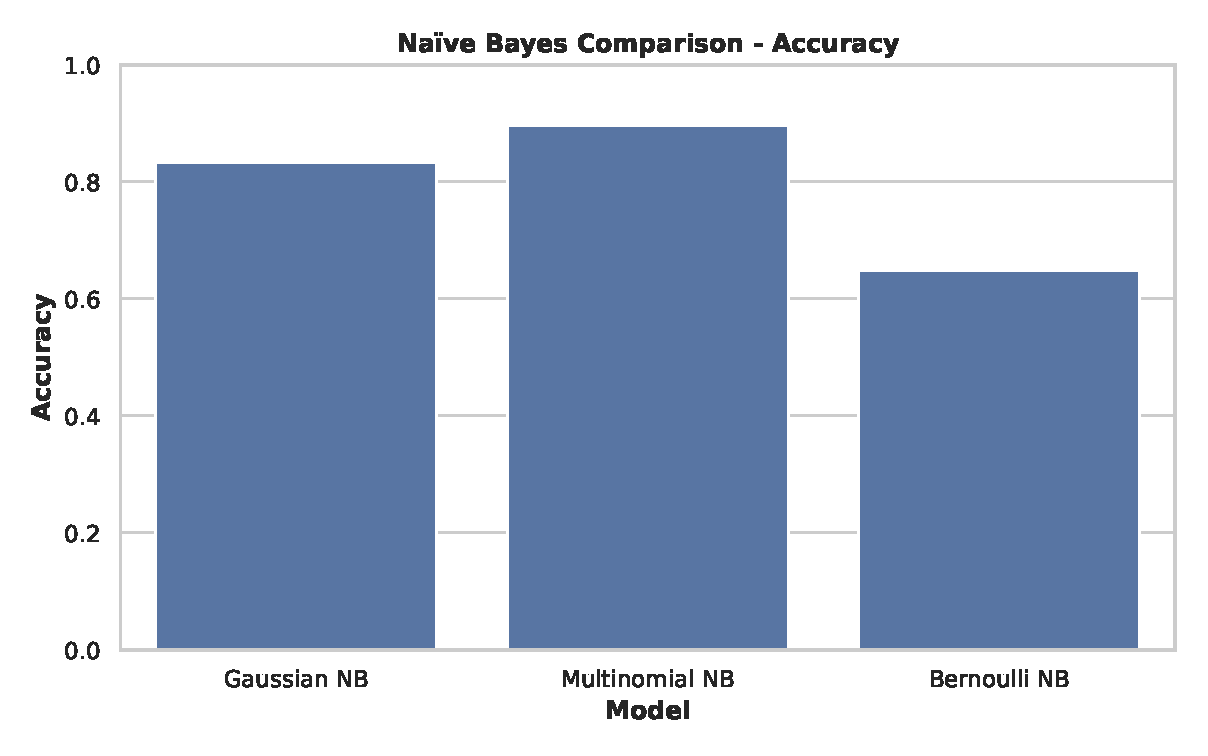
\includegraphics[width=0.9\linewidth]{figures/naive_bayes_accuracy_comparison.eps}
\caption{Test-set accuracy comparison across the three Na\"{\i}ve Bayes variants.}
\end{figure}
 
\begin{figure}[H]
\centering
\includegraphics[width=0.32\linewidth]{figures/confusion_matrix_Gaussian_NB.eps}
\includegraphics[width=0.32\linewidth]{figures/confusion_matrix_Multinomial_NB.eps}
\includegraphics[width=0.32\linewidth]{figures/confusion_matrix_Bernoulli_NB.eps}
\caption{Confusion matrices for Gaussian, Multinomial and Bernoulli NB (left to right).}
\end{figure}

\begin{figure}[H]
\centering
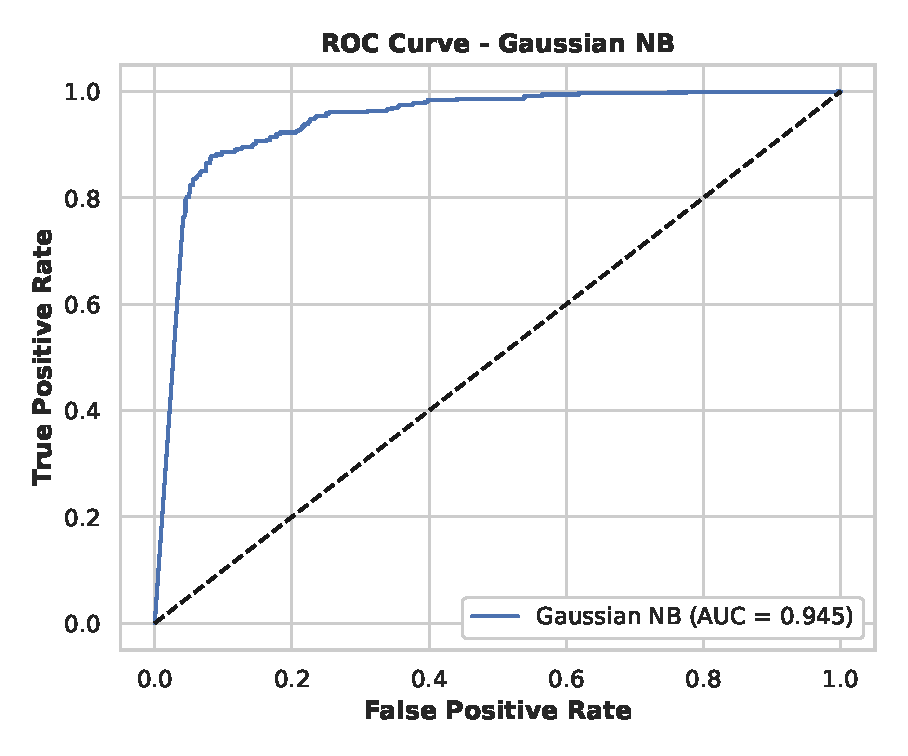
\includegraphics[width=0.32\linewidth]{figures/roc_curve_Gaussian_NB.eps}
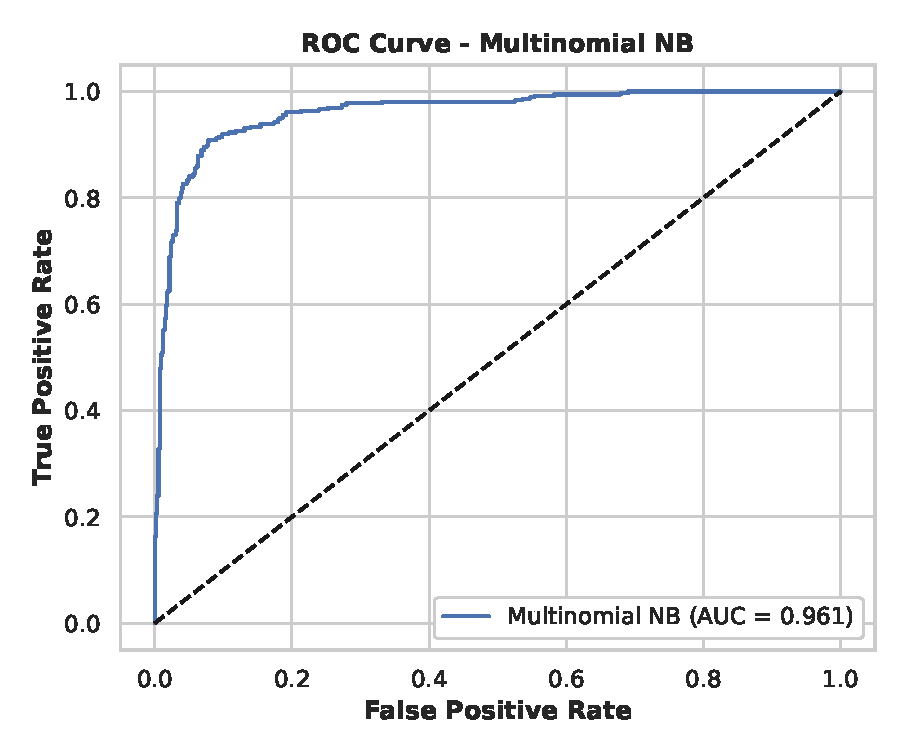
\includegraphics[width=0.32\linewidth]{figures/roc_curve_Multinomial_NB.eps}
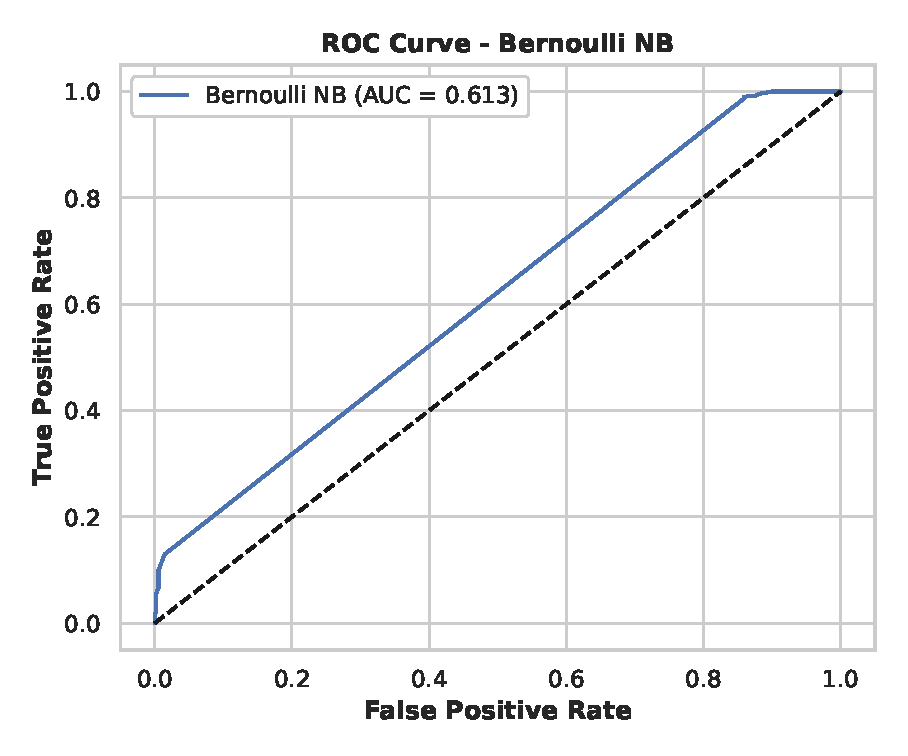
\includegraphics[width=0.32\linewidth]{figures/roc_curve_Bernoulli_NB.eps}
\caption{ROC curves for Gaussian, Multinomial and Bernoulli NB (left to right).}
\end{figure}
 
\begin{figure}[H]
\centering
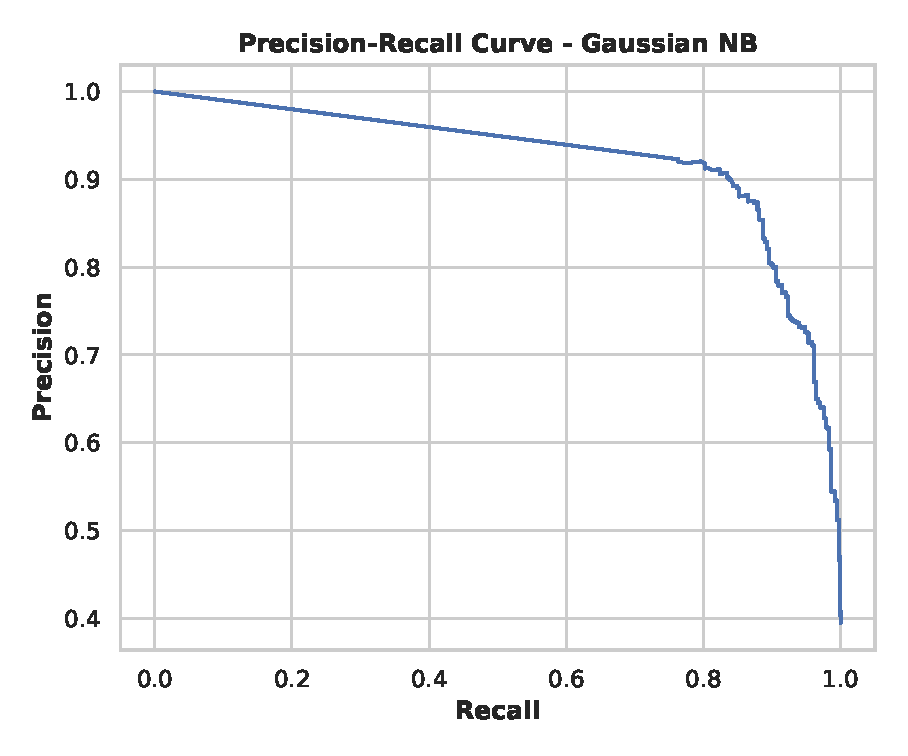
\includegraphics[width=0.32\linewidth]{figures/pr_curve_Gaussian_NB.eps}
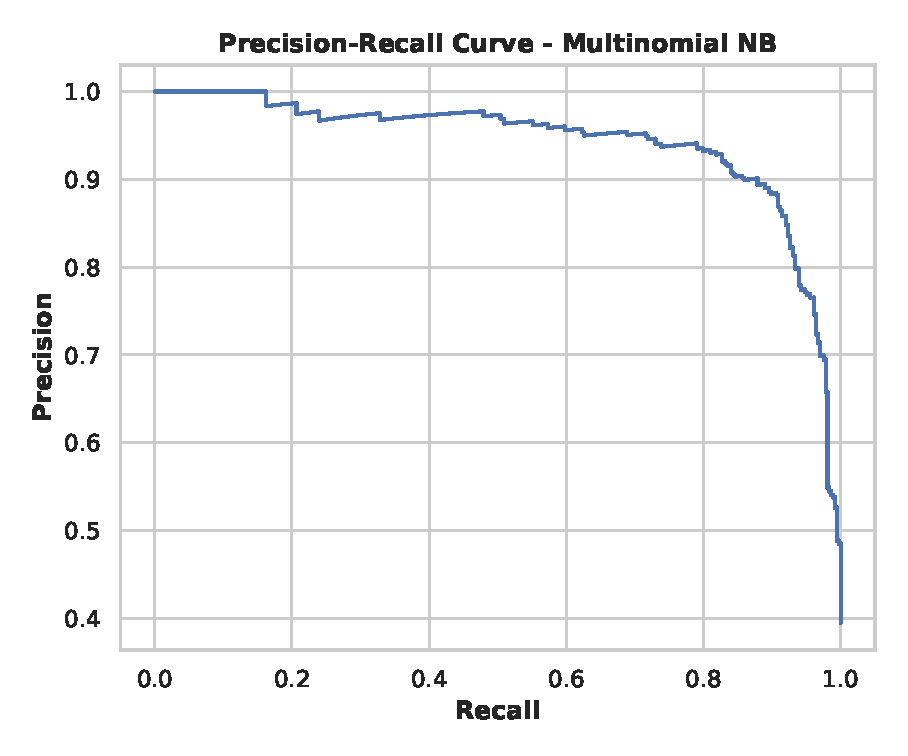
\includegraphics[width=0.32\linewidth]{figures/pr_curve_Multinomial_NB.eps}
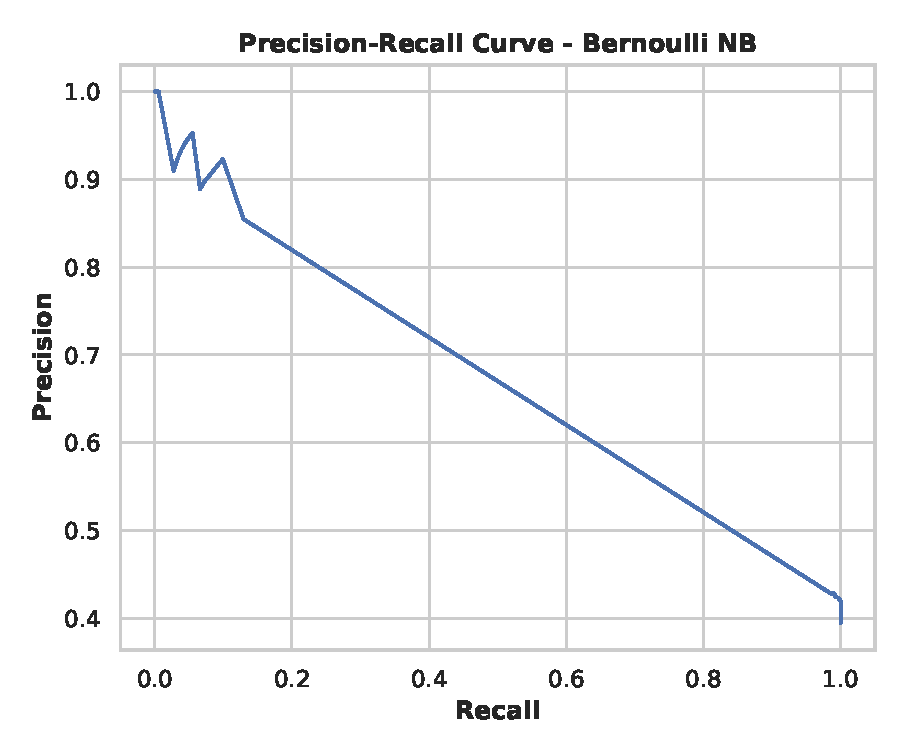
\includegraphics[width=0.32\linewidth]{figures/pr_curve_Bernoulli_NB.eps}
\caption{Precision-Recall curves for Gaussian, Multinomial and Bernoulli NB (left to right).}
\end{figure}
 
\textbf{Inference:} Multinomial NB comes out on top here -- highest accuracy (0.8958), precision (0.9349), and ROC-AUC (0.9612) of the three. That fits the theory from Section~7.1: its multinomial assumption just matches the count/frequency nature of the \texttt{word\_freq\_*} features better than a Gaussian or a hard binary assumption ever could. Gaussian NB, on the other hand, is trading precision for recall -- its confusion matrix shows a lot of ham messages getting misclassified as spam, which isn't great in a real spam filter, since blocking a genuine e-mail is usually worse than letting one spam message through. Bernoulli NB basically falls apart: an ROC-AUC of 0.6135 is barely better than a coin flip, and its 0.6482 accuracy is only a hair above the 60.6\% ``always predict ham'' baseline from Section~4.1. That's a pretty strong confirmation that the fixed 0.5 binarisation threshold is destroying nearly all the useful signal here (see Section~4.3).

\subsection{KNN Performance vs.\ $k$}
 
\begin{figure}[H]
\centering
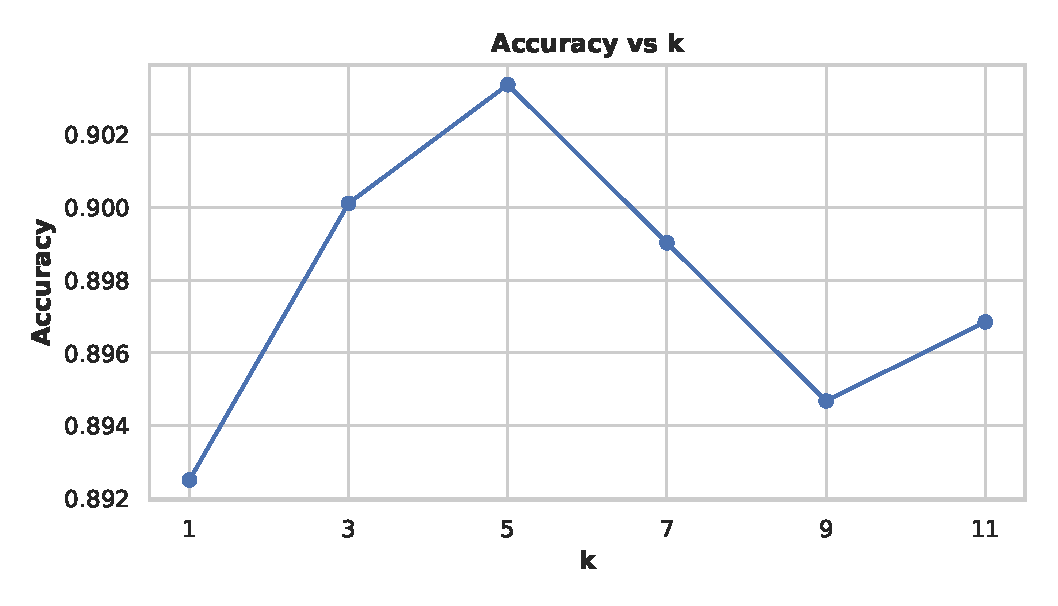
\includegraphics[width=0.7\linewidth]{figures/accuracy_vs_k.eps}
\caption{KNN accuracy as a function of $k$ (uniform weighting, default Euclidean distance).}
\end{figure}
\textbf{Inference:} Accuracy peaks at $k=5$ (0.9034) and drops off a little for larger $k$ -- a fairly textbook bias-variance trade-off. $k=1$ is the most flexible option and has the highest variance, so it gets dragged down by locally noisy neighbours. Very large $k$ does the opposite -- it over-smooths the decision boundary and starts pulling in points from the majority (ham) class, which hurts both accuracy and recall. What's a bit more interesting is that ROC-AUC keeps climbing with $k$ (0.888 at $k=1$, up to 0.954 at $k=11$) even as accuracy falls after $k=5$. One possible explanation is that larger $k$ gives smoother, better-calibrated probability estimates, even though the default 0.5 decision threshold stops being the ideal cut-off for accuracy once the neighbourhood gets that large.
 
\subsection{GridSearchCV vs.\ RandomizedSearchCV}
 
\begin{figure}[H]
\centering
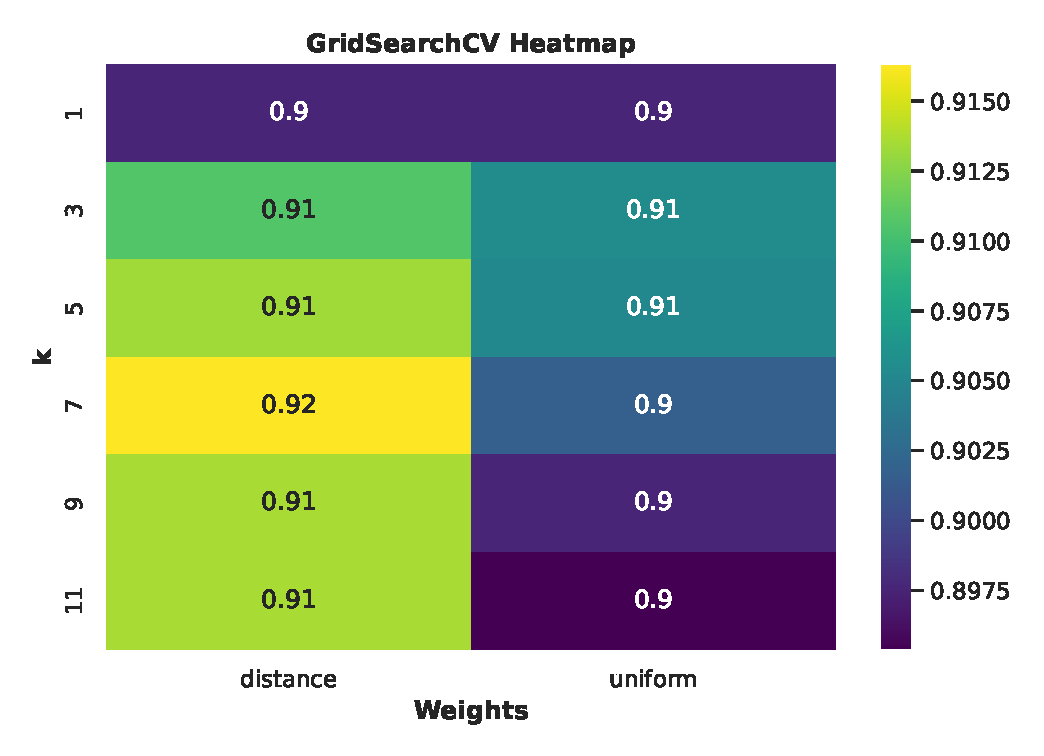
\includegraphics[width=0.6\linewidth]{figures/gridsearch_heatmap.eps}
\caption{GridSearchCV mean CV accuracy across $n\_neighbors$ and $weights$.}
\end{figure}
\begin{figure}[H]
\centering
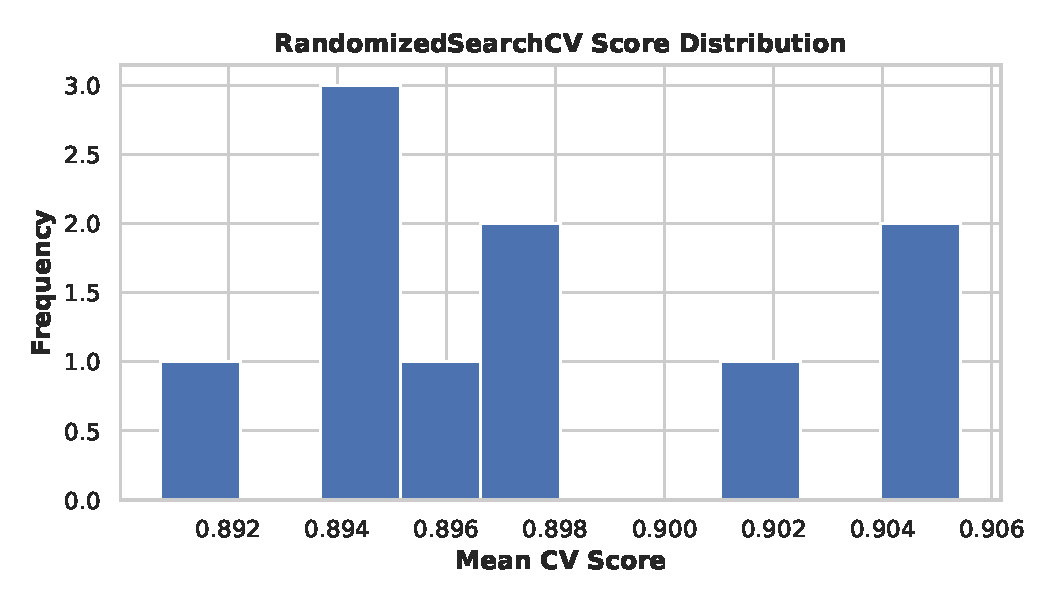
\includegraphics[width=0.6\linewidth]{figures/randomizedsearch_score_distribution.eps}
\caption{Distribution of mean CV scores across the 10 configurations sampled by RandomizedSearchCV.}
\end{figure}
\textbf{Inference:} The exhaustive grid search genuinely found a better configuration than either the manual $k$-sweep (Section~8.2, best test accuracy 0.9034 at $k=5$, uniform weights) or the random search. Distance weighting paired with Manhattan distance ($p=1$) at $k=7$ reached 0.9163 CV accuracy -- roughly a percentage point better. Looking at the heatmap, distance weighting beats uniform weighting across almost every value of $k$ we tried, which backs up the idea that closer neighbours really do carry more reliable information for this dataset. RandomizedSearchCV, having only sampled 10 of the full grid's combinations, ended up with a noticeably weaker setup ($k=3$, uniform, kd\_tree) -- about 1.1 points lower in CV accuracy -- but it got there in 2.16s versus GridSearchCV's 18.08s, roughly an 8.4$\times$ speed-up. That's a fairly classic exhaustive-search-vs-speed trade-off.
 
\subsection{KDTree vs.\ BallTree}

\textbf{Inference:} Accuracy is identical for both trees, which isn't surprising -- both are exact nearest-neighbour structures, so they have to return the same $k$ neighbours as brute force; they just differ in \emph{how} they search, not \emph{what} they find. BallTree came out faster on both build (0.0137s vs.\ 0.0223s) and query (0.1795s vs.\ 0.2151s) for this dataset. This tracks with the theory in Section~7.2: with $d=57$ dimensions, we're already well past the point where KDTree's axis-aligned splitting starts losing its pruning advantage over brute force -- the usual rule of thumb is that KDTrees stop paying off somewhere above roughly 20 dimensions -- whereas BallTree's spherical, metric-based partitioning tends to degrade more gracefully.
 
\subsection{5-Fold Cross Validation}

\begin{figure}[H]
\centering
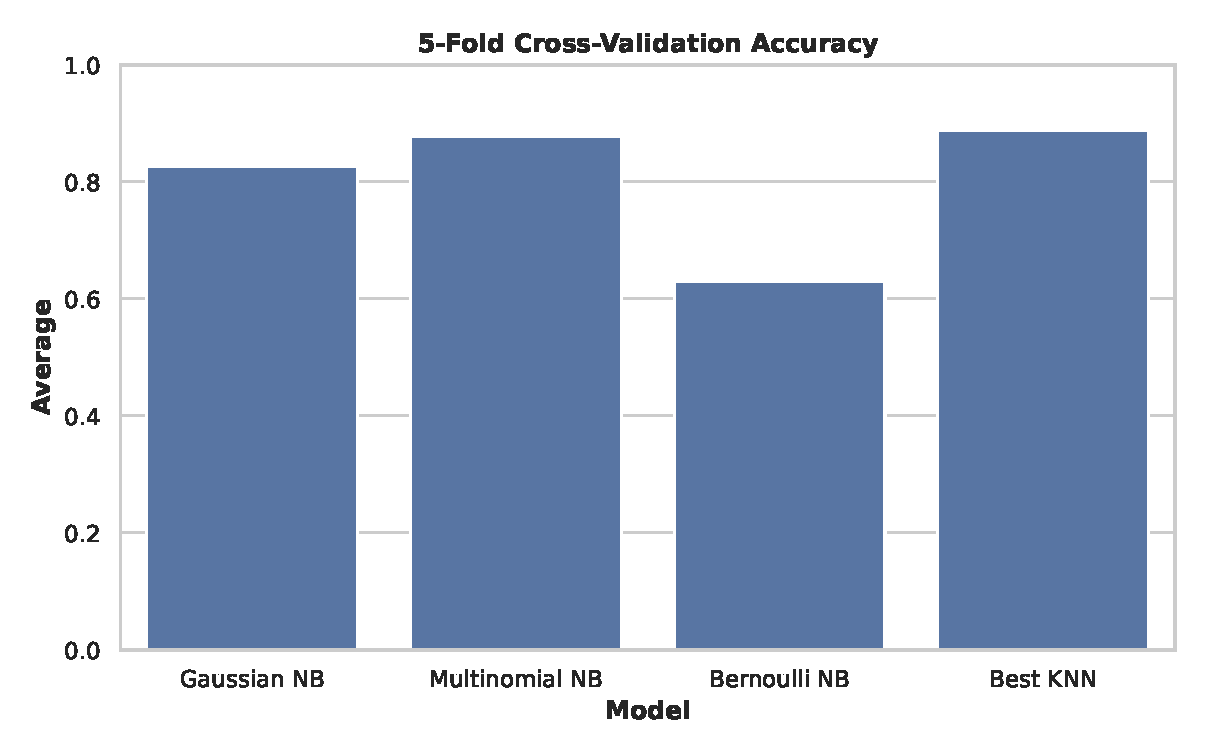
\includegraphics[width=0.7\linewidth]{figures/cross_validation_accuracy.eps}
\caption{5-fold cross-validation accuracy comparison.}
\end{figure}
\textbf{Inference:} The cross-validated ranking (Best KNN $>$ Multinomial $>$ Gaussian $>$ Bernoulli) lines up with the single-split ranking from Sections~8.1--8.2, which is reassuring -- it means the earlier result probably wasn't just a lucky split. Fold~5 is noticeably harder for every model; all four scores dip there, which points to that fold containing an intrinsically harder-to-separate subset of e-mails rather than any one model being unstable. That said, Gaussian NB is hit disproportionately hard, falling all the way to 0.70 (a 12--15 point drop compared to its other folds), while Multinomial NB only dips to 0.8533. We think this out-sized sensitivity ties back to Gaussian NB's distributional mismatch discussed in Section~4.3 -- whichever fold happens to pick up more of the extreme-tail spam messages is going to violate its normality assumption the hardest.
 
\subsection{Final Tuned KNN -- Evaluation}
\begin{figure}[H]
\centering
\includegraphics[width=0.32\linewidth]{figures/confusion_matrix_Best_KNN.eps}
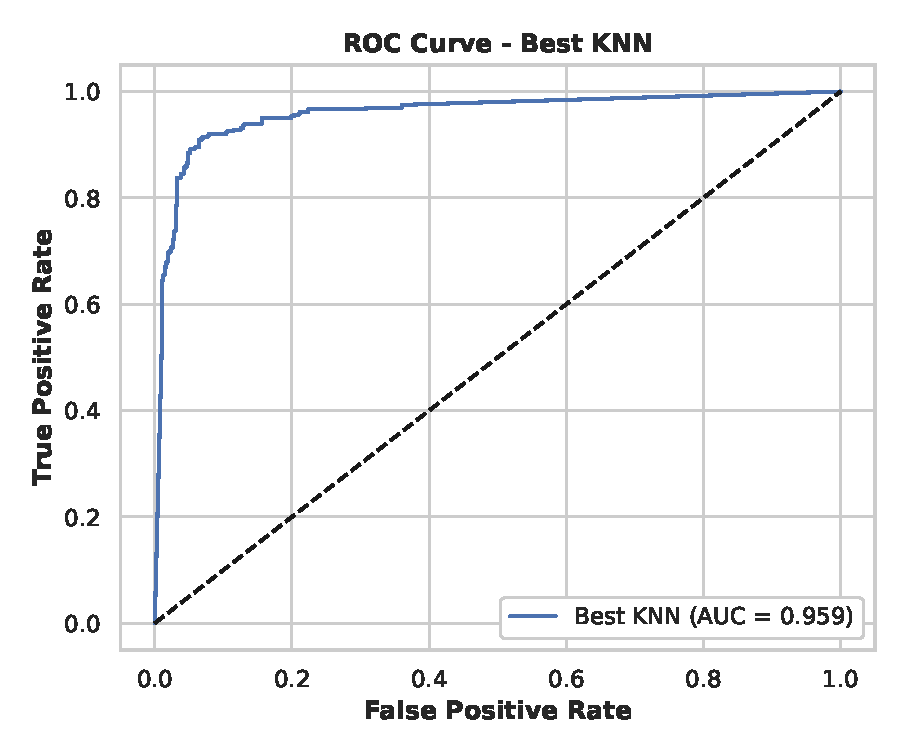
\includegraphics[width=0.32\linewidth]{figures/roc_curve_Best_KNN.eps}
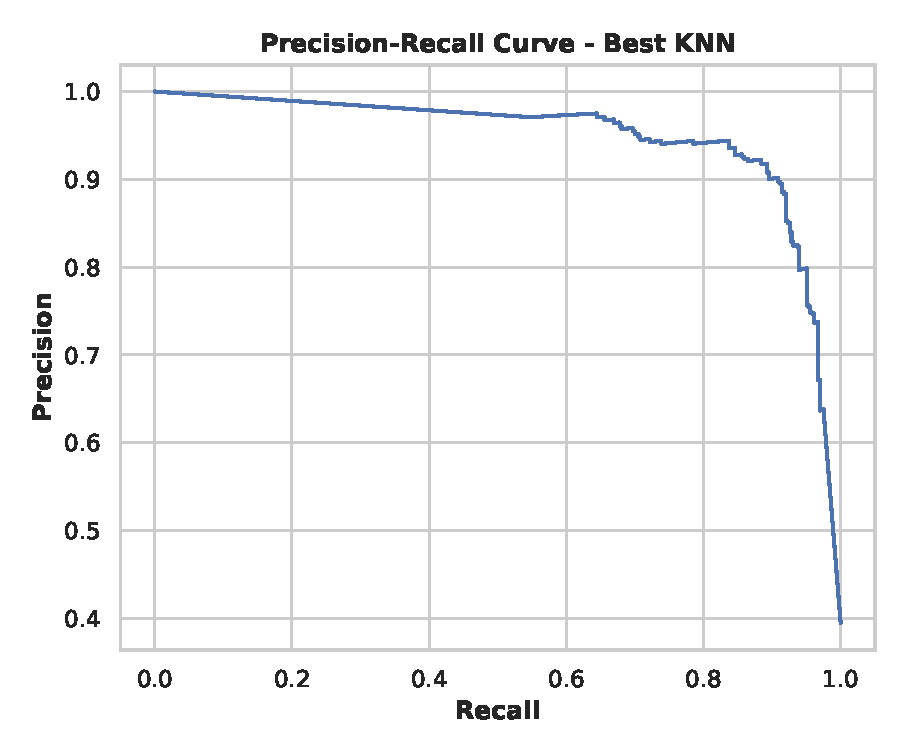
\includegraphics[width=0.32\linewidth]{figures/pr_curve_Best_KNN.eps}
\caption{Confusion matrix, ROC curve and Precision-Recall curve for the GridSearchCV-tuned best KNN model ($k=7$, distance-weighted, Manhattan).}
\end{figure}
\textbf{Inference:} On the held-out test set, the tuned model reaches 0.9175 accuracy -- about 1.4 points above the untuned $k=5$/uniform model's 0.9034 from Section~8.2 -- and this is very close to the 0.9163 accuracy GridSearchCV had already estimated via cross-validation (Section~8.3). The gap there is only about 0.1 points, which is a good sign: it suggests the CV procedure generalised well, and the test-set number can be trusted rather than chalked up to a lucky split.
 
\subsection{Experimental Time Analysis}

\begin{figure}[H]
\centering
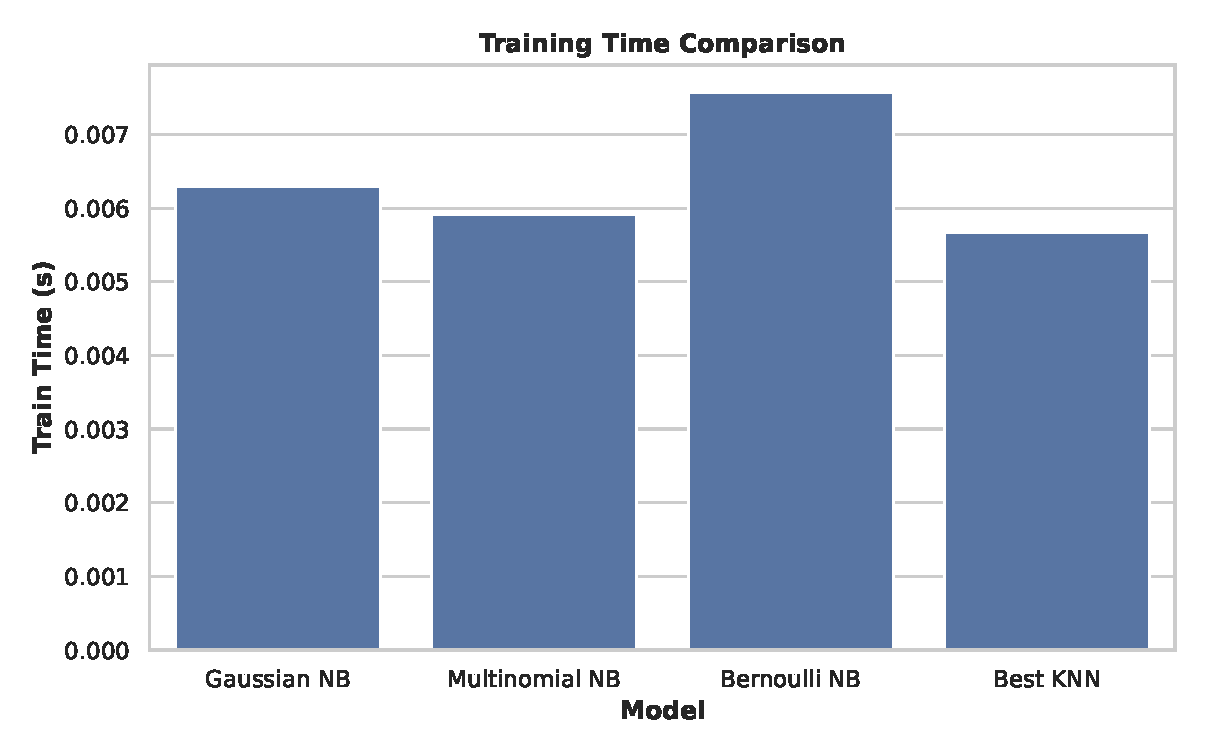
\includegraphics[width=0.48\linewidth]{figures/training_time_comparison.eps}
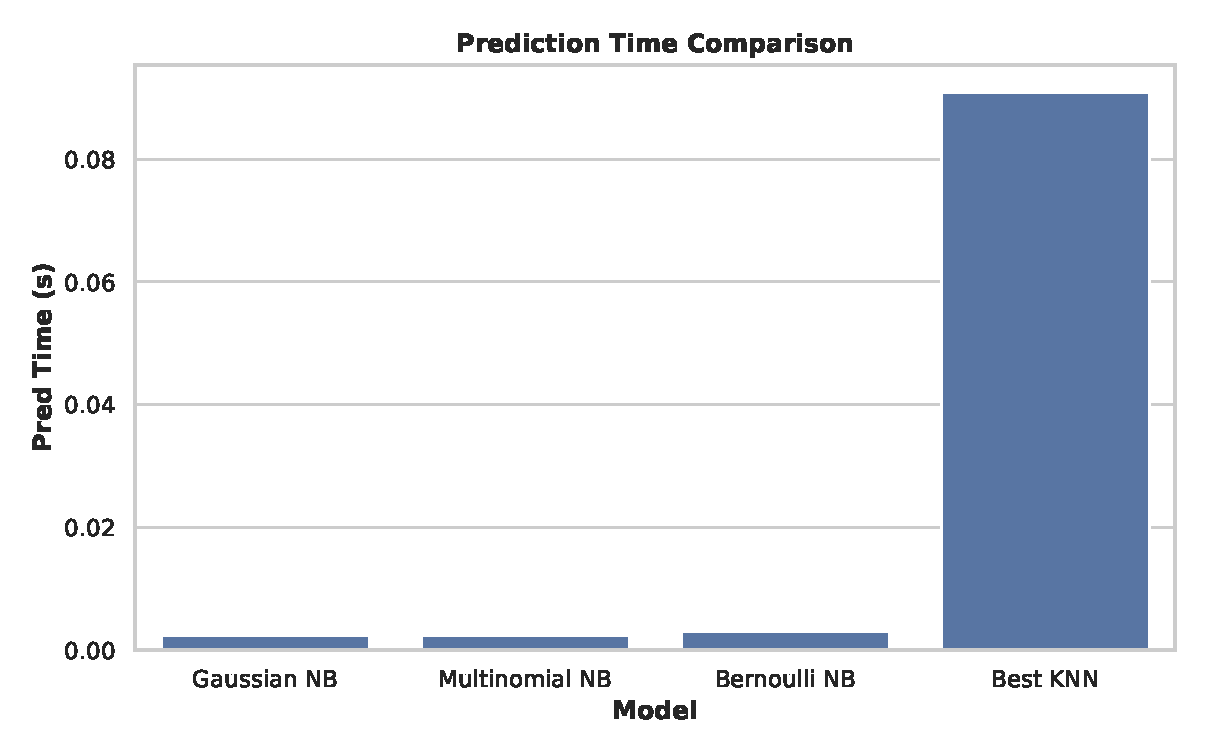
\includegraphics[width=0.48\linewidth]{figures/prediction_time_comparison.eps}
\caption{Training time (left) and prediction time (right) across all four final models.}
\end{figure}
\textbf{Inference:} All four models train in a few milliseconds -- Best KNN is actually the fastest of the four to ``train'' (0.0057s), which makes sense given it's a lazy learner and really just stores the training data. That matches its theoretical $O(1)$ training complexity from Section~8.8. Prediction tells the opposite story, though: Best KNN's prediction time (0.0908s) is roughly 32--40$\times$ slower than any Na\"{\i}ve Bayes variant. That's because GridSearchCV picked \texttt{algorithm='brute'} (Section~8.3), which has to compute the distance to all 3680 training points for every one of the 921 test queries -- an $O(nd)$ cost per prediction batch, right in line with what theory predicts. It's a pretty direct, measured illustration of the training-cost/prediction-cost trade-off between these two algorithm families.

 
\subsection{Final Classifier Comparison}

\begin{figure}[H]
\centering
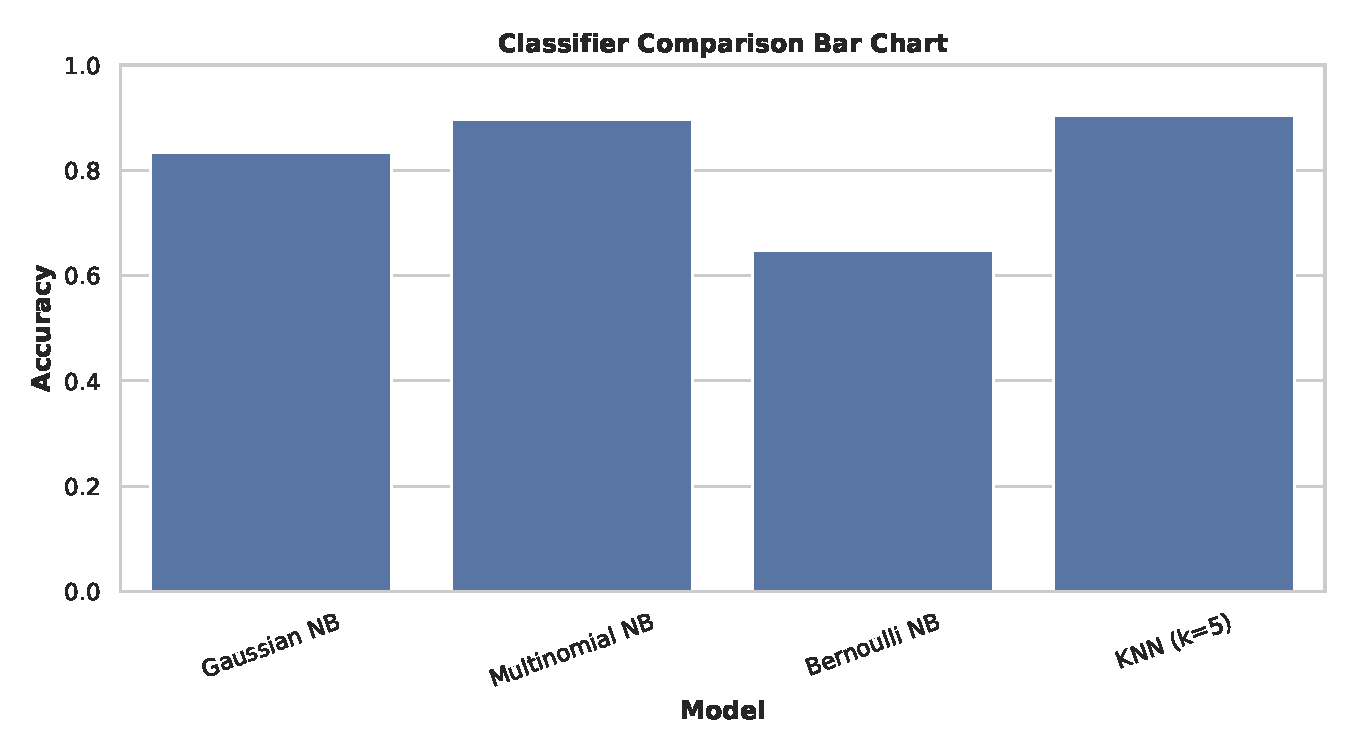
\includegraphics[width=0.75\linewidth]{figures/classifier_comparison_accuracy.eps}
\caption{Final test-set accuracy comparison across all four classifiers.}
\end{figure}
\textbf{Inference:} KNN ($k=5$) edges out Multinomial NB on raw accuracy and F1, but Multinomial NB still wins on precision and ROC-AUC, and does so at a fraction of KNN's prediction cost (Section~8.7). So really, which model is ``best'' depends on what you're optimising for in deployment -- KNN if you want the highest overall correctness, Multinomial NB if you'd rather minimise false alarms and get well-ranked probability scores while spending far less on computation.


\section{Additional Tasks}
 
\subsection{Different Train-Test Splits}
Evaluated using the GridSearchCV-tuned best KNN model ($k=7$, distance-weighted, Manhattan, brute force): \\ \\
\begin{tabular}{lcc}
\toprule
Split (train/test) & Accuracy & F1-Score\\
\midrule
90/10 & 0.9002 & 0.8678 \\
80/20 & 0.9175 & 0.8920 \\
70/30 & 0.9247 & 0.9021 \\
\bottomrule
\end{tabular} \\ \\
\textbf{Inference:} Both accuracy and F1 improve as more data goes into training -- 70/30 gives the tuned KNN model more neighbours to draw on at prediction time -- at the cost of a smaller, higher-variance test set to measure that performance against. The trend keeps climbing rather than levelling off, which suggests the model hadn't fully saturated at 80/20 and could probably benefit from even more training data.
 
\subsection{Euclidean vs.\ Manhattan Distance}
Evaluated at $k=5$ (uniform weights, \texttt{algorithm='auto'}): \\ \\
\begin{tabular}{lcc}
\toprule
Distance & Accuracy & F1-Score\\
\midrule
Manhattan ($p=1$) & 0.9045 & 0.8736 \\
Euclidean ($p=2$) & 0.9034 & 0.8762 \\
\bottomrule
\end{tabular} \\ \\
\textbf{Inference:} The two metrics perform almost identically -- within 0.1--0.3 points of each other -- with Manhattan a touch ahead on accuracy and Euclidean a touch ahead on F1. Given that GridSearchCV also independently landed on $p=1$ (Manhattan) as part of its best configuration (Section~8.3), this near-tie makes us think the distance-metric choice is a fairly minor factor here compared to $k$ and the weighting scheme.
 
\subsection{Weighted vs.\ Uniform KNN}
Evaluated at $k=5$: \\
\begin{tabular}{lcc}
\toprule
Weighting & Accuracy & F1-Score\\
\midrule
Uniform  & 0.9034 & 0.8762 \\
Distance & 0.9077 & 0.8821 \\
\bottomrule
\end{tabular} \\ \\
\textbf{Inference:} Distance weighting improves both accuracy (+0.43 points) and F1 (+0.59 points) over uniform voting at the same $k$, which lines up with the same effect that led GridSearchCV to pick distance weighting overall (Section~8.3). It seems like weighting down the influence of farther neighbours mostly helps points sitting near the ham/spam decision boundary, where uniform voting is easier to sway by a majority of merely-nearby-but-not-closest neighbours.
 
\subsection{Overfitting/Underfitting Discussion}
The $k$-sweep in Section~8.2 shows both regimes pretty clearly. $k=1$ overfits -- it follows the training data (noise included) so closely that it's actually the worst performer on the test set (0.8925 accuracy, lowest ROC-AUC at 0.8882), despite having zero bias toward any particular neighbourhood shape. At the other end, large $k$ (9, 11) starts to underfit with respect to accuracy: the decision rule increasingly just reflects the global class prior (60.6\% ham) instead of local structure, so recall for the minority spam class drops (0.8540 at $k=9$, 0.8512 at $k=11$, versus 0.8678 at the optimal $k=5$). $k=5$ looks like the closest thing to a bias-variance sweet spot for raw accuracy on this feature space, though Section~8.3 shows that once distance weighting enters the picture, that sweet spot shifts slightly, to $k=7$.
 
\section{Discussion}
 
\subsection*{Analysis Questions}
\begin{enumerate}[leftmargin=*]
\item \textbf{Which Na\"{\i}ve Bayes variant performed best?} Multinomial NB, by a fair margin -- highest accuracy (0.8958), precision (0.9349) and ROC-AUC (0.9612) of the three (Section~8.1). Its count-based assumption just matches the \texttt{word\_freq\_*} features much better than either Gaussian NB's normality assumption or Bernoulli NB's hard binarisation.
\item \textbf{What is the optimal value of $k$?} In the plain uniform-weighted sweep, $k=5$ gave the best test accuracy (0.9034, Section~8.2). Once distance weighting and the Manhattan metric are also tuned, though, GridSearchCV found $k=7$ to be jointly optimal (CV accuracy 0.9163, Section~8.3) -- so really, ``best $k$'' depends on the weighting scheme you're using.
\item \textbf{Compare GridSearchCV and RandomizedSearchCV.} GridSearchCV exhaustively worked through the full 36-combination grid and found a genuinely better configuration (0.9163 CV accuracy) than RandomizedSearchCV's 10 sampled combinations (0.9054) -- but it took roughly 8.4$\times$ longer to do it (18.08s vs.\ 2.16s, Section~8.3).
\item \textbf{Compare KDTree and BallTree.} Same accuracy for both, since they're both exact search structures, but BallTree was quicker to build and query on this 57-dimensional dataset (Section~8.4), which fits with KDTree's known weakness in higher dimensions.
\item \textbf{Compare theoretical and practical complexity.} The measured times lined up well with theory: KNN's near-zero training time confirmed the expected $O(1)$ training complexity, and its noticeably slower prediction time (0.0908s, roughly 32--40$\times$ the Na\"{\i}ve Bayes models) confirmed the $O(nd)$ brute-force prediction cost, since GridSearchCV's chosen model used \texttt{algorithm='brute'} (Section~8.7).
\item \textbf{Which classifier is preferred for large datasets?} Na\"{\i}ve Bayes, and Multinomial NB in particular, scales better -- its prediction cost is $O(d)$ and doesn't depend on the number of training points $n$, while brute-force KNN's prediction cost grows linearly with $n$. Even tree-based KNN still carries a much bigger constant factor in practice (Section~8.7), so for very large datasets, Multinomial NB's small hit in accuracy/ROC-AUC compared to KNN is usually a reasonable price to pay for the big gain in prediction throughput.
\end{enumerate}
 
Stepping back from the specific questions, two things stood out to us over the course of this experiment. First, feature-distribution assumptions seem to matter a lot more than search-strategy tuning -- the single biggest swing in this whole report was between Na\"{\i}ve Bayes variants (0.6482 up to 0.8958 accuracy, purely from which likelihood model was assumed), while even the most exhaustive KNN hyperparameter search only bought about 1.4 points over a simple $k$-sweep. Second, accuracy alone would have completely hidden Bernoulli NB's near-random ranking ability (ROC-AUC 0.6135) -- tracking ROC-AUC and the Precision-Recall curve throughout was what actually caught that failure, given the class imbalance we noted back in Section~4.1.
 
\section{Conclusion}
We built, tuned, and compared four classifiers -- Gaussian NB, Multinomial NB, Bernoulli NB and KNN -- on the 4601-sample Spambase dataset. Multinomial NB turned out to be the strongest Na\"{\i}ve Bayes variant, and a distance-weighted, Manhattan-metric KNN with $k=7$ (found via GridSearchCV) ended up the overall strongest single model on the test set (0.9175 accuracy) -- narrowly ahead of Multinomial NB on accuracy, but behind it on precision and ROC-AUC, and roughly 32--40$\times$ slower to query. KDTree and BallTree gave identical accuracy but different speeds, with BallTree the better pick at this dataset's dimensionality. GridSearchCV beat RandomizedSearchCV on accuracy, though at a considerable time cost, and 5-fold cross-validation confirmed these rankings held up across different splits rather than being an artefact of one particular train/test partition. All told, choosing between the Na\"{\i}ve Bayes family and KNN for a real spam-filtering deployment should come down to more than raw accuracy -- prediction latency and the relative cost of false positives versus false negatives matter just as much.
 
\section{References}
\begin{enumerate}[leftmargin=*]
\item Scikit-learn Developers, ``Scikit-learn: Machine Learning in Python -- Documentation,'' [Online]. Available: \url{https://scikit-learn.org/stable/documentation.html}.
\item A. G\'eron, \textit{Hands-On Machine Learning with Scikit-Learn, Keras and TensorFlow}, 3rd ed. Sebastopol, CA, USA: O'Reilly Media, 2022.
\item C. M. Bishop, \textit{Pattern Recognition and Machine Learning}. New York, NY, USA: Springer, 2006.
\item M. Hopkins, E. Reeber, G. Forman, and J. Suermondt, ``Spambase Data Set,'' UCI Machine Learning Repository, 1999. [Online]. Available: \url{https://archive.ics.uci.edu/ml/datasets/spambase}.
\end{enumerate}
 
\end{document}